\documentclass{beamer}

\title{``The one" means sigma above average}
\author{Davi Costa}
\institute{Enrico Fermi Institute \& Kadanoff Center for Theoretical Physics,\\ University of Chicago}
\date{February 2, 2023}

\begin{document}

\frame{\titlepage}

\begin{frame}
\frametitle{Should I get married?}
How much should I like my partner to get married? Need to resolve the trade-off of not getting married:

\begin{itemize}
    \item Possibility of finding a better match;
    \item Being dumped by partner because it did.
\end{itemize}


\end{frame}


\begin{frame}
\frametitle{Input: The affinitiy matrix}

\begin{align}
    \textrm{Affinity matrix:} A_{ij}\sim \textrm{Distribution},\qquad 1\leq i,j\leq N
\end{align}

\begin{figure}
  \centering
  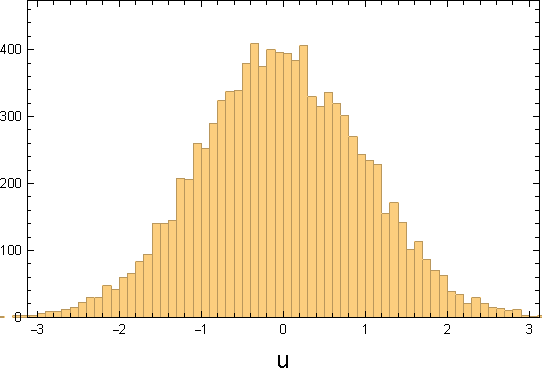
\includegraphics[width=0.6\textwidth]{Ginitialhistogram.pdf}
  \caption{Histogram of the values $\{A_{kj}: 1 \geq j\geq N\}$ of the affinity matrix for some agent $k$ in the Gaussian model $\mathcal{N}(0,1)$.}
  \label{InitialGaussianHistogram}
\end{figure}
\end{frame}



\begin{frame}
\frametitle{Dynamics of the model}




\begin{itemize}
    \item Random matching:
\begin{align}
    \mu_t:\{1,2,\dots,N\} & \rightarrow \{1,2,\dots,N\}
    \label{matching}
\end{align}
    \item Single's evolution: $u_t^k=A_{kk}$, $l=\mu_{t+1}(k)$:
\begin{align}
    u_{t+1}^k=\begin{cases} A_{kl}, & A_{kl}>u_t^k=A_{kk}\ \textrm{and }\ A_{lk}>u_{t}^l,\\
    u_t^k, & \textrm{otherwise}.
    \end{cases}
    \label{singleevolution}
\end{align}

    \item Couple's evolution: $u_t^k=A_{km}$ and $u_t^m=A_{mk}$, match $l=\mu_{t+1}(k)$ and $n=\mu_{t+1}(m)$:
\begin{align}
    u_{t+1}^k=\begin{cases} A_{kl}, & \textrm{if}\quad A_{kl}>u_t^k\ \textrm{and }\ A_{lk}>u_{t}^l,\\
    A_{kk}, & \textrm{if}\quad A_{mn}>u_t^m\ \textrm{and }\ A_{nm}>u_t^n,\\
    u_t^k, & \textrm{otherwise}.
    \end{cases}
    \label{coupleevolution}
\end{align}
\end{itemize}
\end{frame}


\begin{frame}
\frametitle{Quantity of interest: average utility}

\begin{figure}[H]
    \centering
    \begin{minipage}{0.49\textwidth}
        \centering
        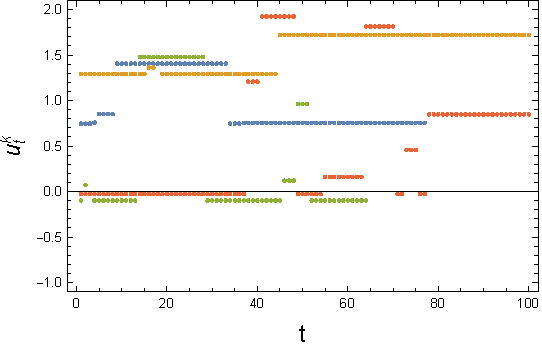
\includegraphics[width=\textwidth]{uktGn10000s1l1.pdf} % first figure itself
        \caption{Evolution of the utility of four agents, distinguished by color, in the Gaussian model $\mathcal{N}(0,1)$ with $N=10.000$}
        \label{uktGn10000s1l1}
    \end{minipage}\hfill
    \begin{minipage}{0.49\textwidth}
        \centering
        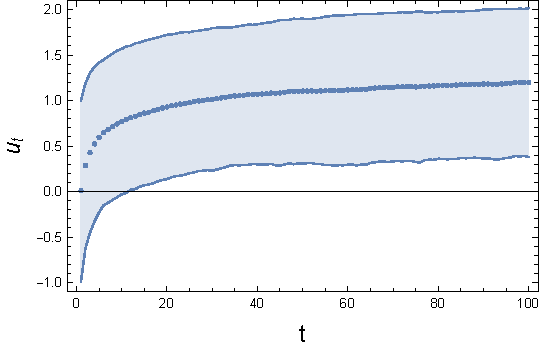
\includegraphics[width=\textwidth]{utGn10000s1l1.pdf}
        \caption{Evolution of average utility with band equal to the variance in the Gaussian model $\mathcal{N}(0,1)$ with $N=10.000$}
        \label{utGn10000s1l1}
    \end{minipage}
\end{figure}
\end{frame}



\begin{frame}{Marriage: proposal vector and new dynamics}
    
\begin{align}
    \textrm{Proposal vector}: \Lambda_{k}\sim \textrm{Distribution},\qquad 1\leq k\leq N
\end{align}

    The $(k,l)$-couple is married at $t$ if

\begin{align}
     u^k_t=A_{kl}>\Lambda_k\qquad \textrm{and}\qquad u^l_t=A_{lk}>\Lambda_k.
    \label{marriedcoupled}
\end{align}


\begin{align}
    \mu_t^\Lambda:\{1,2,\dots,N\}-\mathcal{M}_{t-1}\rightarrow\{1,2,\dots,N\}-\mathcal{M}_{t-1},
    \label{marriedcouples}
\end{align}
\end{frame}


\begin{frame}{Symmetries of the model}
    \begin{itemize}
        \item Without marriage:
    \begin{itemize}
        \item $A_{ij}>A_{kl}$ is preserved by $A_{ij}\rightarrow\tilde{A}_{ij}=\sigma A_{ij}+\mu$
        \item $\mathcal{N}(0,1)\rightarrow \mathcal{N}(\mu,\sigma)$
        \item if $(\mu=0,\sigma=1)\mapsto u_t^k$ then $(\mu,\sigma)\mapsto \sigma u_t^k+\mu$.
    \end{itemize}
        \item With marriage:
        \begin{itemize}
            \item Similar to before but one should shift and re-scale $\Lambda$, so
            \item if $(\mu=0,\sigma=1,\delta)\mapsto u_t^k$ then $(\mu,\sigma,\Lambda)\mapsto \sigma u_t^k+\mu$.
            \item just one parameter to explore: $\delta=\frac{\Lambda-\mu}{\sigma}$.
        \end{itemize}
    \end{itemize}
\end{frame}



\begin{frame}{Results: ``the one" means sigma above average}
    

\begin{figure}[H]
    \centering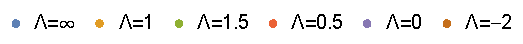
\includegraphics{legend.pdf}
    \begin{minipage}{0.49\textwidth}
        \centering
        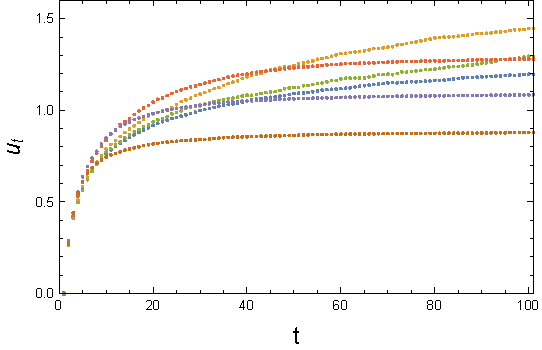
\includegraphics[width=\textwidth]{GLcompN10000s1.pdf} % first figure itself
        \label{uktGn10000s1l1}
    \end{minipage}\hfill
    \begin{minipage}{0.49\textwidth}
        \centering
        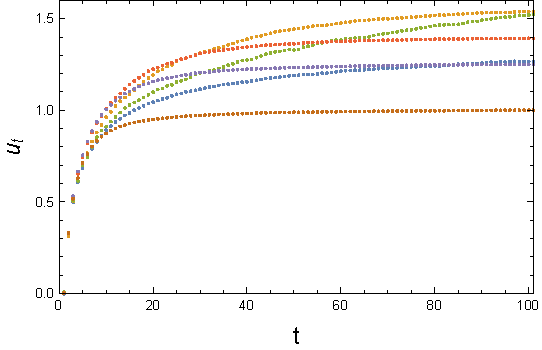
\includegraphics[width=\textwidth]{NewlcompUN10000s1.pdf}
    \end{minipage}
    \caption{Average utility evolution in the Gaussian and Uniform model with $N=10.000$ for different values of $\Lambda$.}
\end{figure}
\end{frame}


\begin{frame}{Results: ``the one" means sigma above average}
    

\begin{figure}[H]
    \centering
    \begin{minipage}{0.49\textwidth}
        \centering
        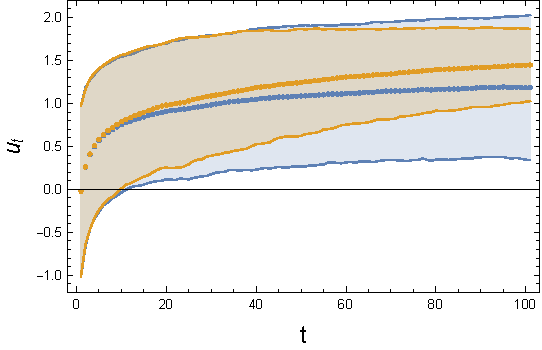
\includegraphics[width=\textwidth]{NewutumtGN10000s1l1.pdf} % first figure itself
        \label{uktGn10000s1l1}
    \end{minipage}\hfill
    \begin{minipage}{0.49\textwidth}
        \centering
        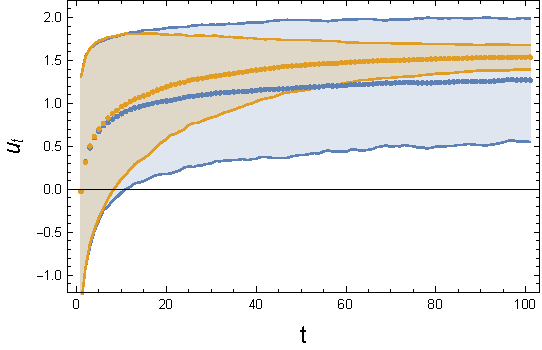
\includegraphics[width=\textwidth]{NewutumtUN10000s1l1.pdf}
    \end{minipage}
    \caption{Average utility evolution in the the system with marriage and $\Lambda=1$ (orange) and without marriage (blue) in the Gaussian and Uniform models.}
\end{figure}
\end{frame}


\begin{frame}{Results: changing the single average}
    

\begin{figure}[H]
    \centering
    \begin{minipage}{0.49\textwidth}
        \centering
        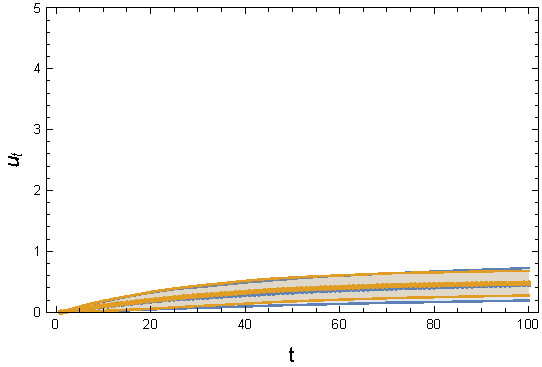
\includegraphics[width=\textwidth]{mum1.pdf} % first figure itself
        \label{uktGn10000s1l1}
    \end{minipage}\hfill
    \begin{minipage}{0.49\textwidth}
        \centering
        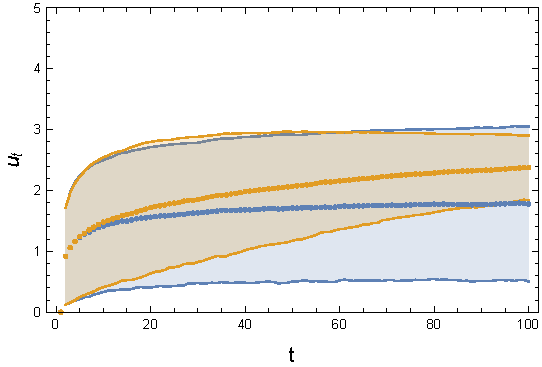
\includegraphics[width=\textwidth]{mu1.pdf}
    \end{minipage}
    \caption{Average utility evolution for $A_{kk}=0$ and $A_{ij}\sim\mathcal{N}(\mu,1)$.}
\end{figure}
\end{frame}



\begin{frame}{Results: comparison with data}
    
\begin{figure}[H]
    \centering
    \begin{minipage}{0.47\textwidth}
        \centering
        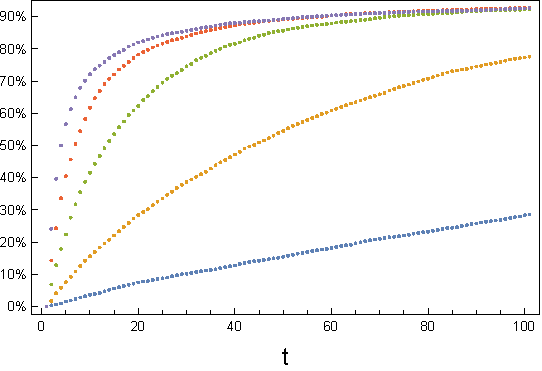
\includegraphics[width=\textwidth]{mclcompUN10000s1.pdf}
        \caption{Share of married agents for different values of $\Lambda$.}
        \label{mcsimulation}
    \end{minipage}\hfill
    \begin{minipage}{0.47\textwidth}
        \centering
        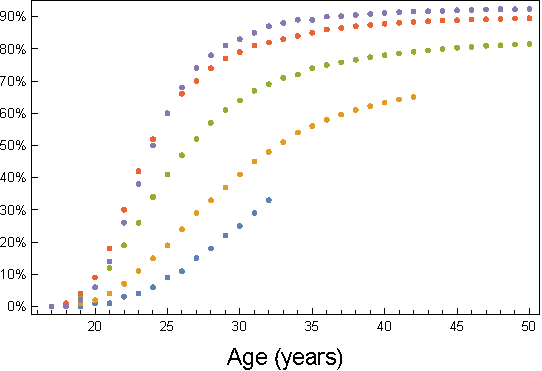
\includegraphics[width=\textwidth]{mcrealdata.pdf}
        \caption{Share of men in England and Wales who were married by a certain age.}
        \label{mcrealdata}
    \end{minipage}
\end{figure}

From bottom to the upper lines the plots corresponds respectively to: $\Lambda=1.5,1,0.5,0,-2$ and men born at $1980,1970,1960,1950,1940$
\end{frame}

\begin{frame}{Results: miscellaneous}

    \begin{itemize}
        \item Gap is smaller for people that are liked more;
        \item $u_{\textrm{Gale}-\textrm{Shapley}}\sim 4u$;
        \item Results stil holds if one partition the society into groups: e.g., men and women;
        \item Having dynamical preferences will automatically add ``divorce" to the model.
    \end{itemize}
\end{frame}







\end{document}